\begin{figure}[htbp]
\centering
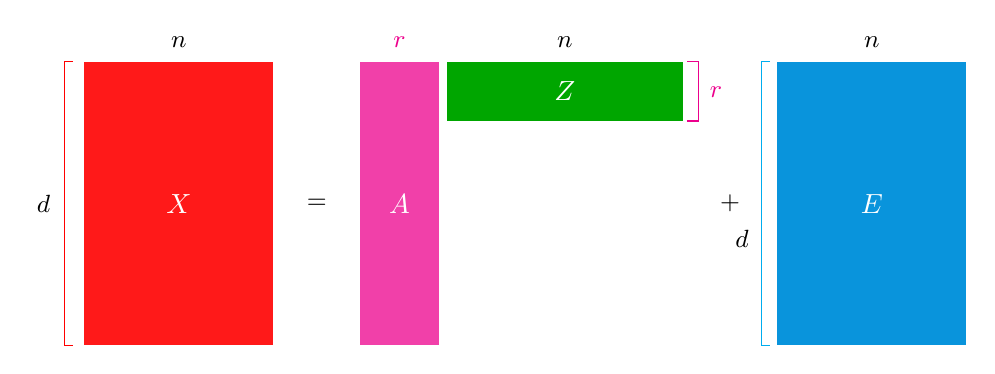
\begin{tikzpicture}[x=1cm,y=1cm,font=\small]
\fill[red!90] (.6,0) rectangle (3,3.6);
\fill[magenta!75] (4.1,0) rectangle (5.1,3.6);
\fill[green!65!black] (5.2,2.85) rectangle (8.2,3.6);
\fill[cyan!80!blue] (9.4,0) rectangle (11.8,3.6);
\node[text=white,font=\bfseries] at (1.8,1.8) {$X$};
\node[text=white,font=\bfseries] at (4.6,1.8) {$A$};
\node[text=white,font=\bfseries] at (6.7,3.23) {$Z$};
\node[text=white,font=\bfseries] at (10.6,1.8) {$E$};
\node at (3.55,1.8) {$=$};\node at (8.8,1.8) {$+$};
\node at (1.8,3.85) {$n$};\node[text=magenta] at (4.6,3.85) {$r$};
\node at (6.7,3.85) {$n$};\node at (10.6,3.85) {$n$};
\draw[red] (.45,0)--(.35,0)--(.35,3.6)--(.45,3.6);\node at (.08,1.8) {$d$};
\draw[magenta] (8.25,2.85)--(8.4,2.85)--(8.4,3.6)--(8.25,3.6);\node[text=magenta] at (8.62,3.22) {$r$};
\draw[cyan] (9.3,0)--(9.2,0)--(9.2,3.6)--(9.3,3.6);\node at (8.95,1.35) {$d$};
\end{tikzpicture}
\origfig{21}{低秩模型。}
\label{fig:ch04a-21}
\end{figure}
